% Options for packages loaded elsewhere
\PassOptionsToPackage{unicode}{hyperref}
\PassOptionsToPackage{hyphens}{url}
\PassOptionsToPackage{dvipsnames,svgnames,x11names}{xcolor}
%
\documentclass[
  11pt,
]{article}

\usepackage{amsmath,amssymb}
\usepackage{setspace}
\usepackage{iftex}
\ifPDFTeX
  \usepackage[T1]{fontenc}
  \usepackage[utf8]{inputenc}
  \usepackage{textcomp} % provide euro and other symbols
\else % if luatex or xetex
  \usepackage{unicode-math}
  \defaultfontfeatures{Scale=MatchLowercase}
  \defaultfontfeatures[\rmfamily]{Ligatures=TeX,Scale=1}
\fi
\usepackage{lmodern}
\ifPDFTeX\else  
    % xetex/luatex font selection
    \setmainfont[]{Arial}
    \setmonofont[]{DejaVu Sans Mono}
\fi
% Use upquote if available, for straight quotes in verbatim environments
\IfFileExists{upquote.sty}{\usepackage{upquote}}{}
\IfFileExists{microtype.sty}{% use microtype if available
  \usepackage[]{microtype}
  \UseMicrotypeSet[protrusion]{basicmath} % disable protrusion for tt fonts
}{}
\makeatletter
\@ifundefined{KOMAClassName}{% if non-KOMA class
  \IfFileExists{parskip.sty}{%
    \usepackage{parskip}
  }{% else
    \setlength{\parindent}{0pt}
    \setlength{\parskip}{6pt plus 2pt minus 1pt}}
}{% if KOMA class
  \KOMAoptions{parskip=half}}
\makeatother
\usepackage{xcolor}
\usepackage[lmargin=0.8in,rmargin=0.8in,tmargin=0.8in,bmargin=0.8in]{geometry}
\ifLuaTeX
  \usepackage{luacolor}
  \usepackage[soul]{lua-ul}
\else
  \usepackage{soul}
  
\fi
\setlength{\emergencystretch}{3em} % prevent overfull lines
\setcounter{secnumdepth}{-\maxdimen} % remove section numbering
% Make \paragraph and \subparagraph free-standing
\makeatletter
\ifx\paragraph\undefined\else
  \let\oldparagraph\paragraph
  \renewcommand{\paragraph}{
    \@ifstar
      \xxxParagraphStar
      \xxxParagraphNoStar
  }
  \newcommand{\xxxParagraphStar}[1]{\oldparagraph*{#1}\mbox{}}
  \newcommand{\xxxParagraphNoStar}[1]{\oldparagraph{#1}\mbox{}}
\fi
\ifx\subparagraph\undefined\else
  \let\oldsubparagraph\subparagraph
  \renewcommand{\subparagraph}{
    \@ifstar
      \xxxSubParagraphStar
      \xxxSubParagraphNoStar
  }
  \newcommand{\xxxSubParagraphStar}[1]{\oldsubparagraph*{#1}\mbox{}}
  \newcommand{\xxxSubParagraphNoStar}[1]{\oldsubparagraph{#1}\mbox{}}
\fi
\makeatother

\usepackage{color}
\usepackage{fancyvrb}
\newcommand{\VerbBar}{|}
\newcommand{\VERB}{\Verb[commandchars=\\\{\}]}
\DefineVerbatimEnvironment{Highlighting}{Verbatim}{commandchars=\\\{\}}
% Add ',fontsize=\small' for more characters per line
\usepackage{framed}
\definecolor{shadecolor}{RGB}{241,243,245}
\newenvironment{Shaded}{\begin{snugshade}}{\end{snugshade}}
\newcommand{\AlertTok}[1]{\textcolor[rgb]{0.68,0.00,0.00}{#1}}
\newcommand{\AnnotationTok}[1]{\textcolor[rgb]{0.37,0.37,0.37}{#1}}
\newcommand{\AttributeTok}[1]{\textcolor[rgb]{0.40,0.45,0.13}{#1}}
\newcommand{\BaseNTok}[1]{\textcolor[rgb]{0.68,0.00,0.00}{#1}}
\newcommand{\BuiltInTok}[1]{\textcolor[rgb]{0.00,0.23,0.31}{#1}}
\newcommand{\CharTok}[1]{\textcolor[rgb]{0.13,0.47,0.30}{#1}}
\newcommand{\CommentTok}[1]{\textcolor[rgb]{0.37,0.37,0.37}{#1}}
\newcommand{\CommentVarTok}[1]{\textcolor[rgb]{0.37,0.37,0.37}{\textit{#1}}}
\newcommand{\ConstantTok}[1]{\textcolor[rgb]{0.56,0.35,0.01}{#1}}
\newcommand{\ControlFlowTok}[1]{\textcolor[rgb]{0.00,0.23,0.31}{\textbf{#1}}}
\newcommand{\DataTypeTok}[1]{\textcolor[rgb]{0.68,0.00,0.00}{#1}}
\newcommand{\DecValTok}[1]{\textcolor[rgb]{0.68,0.00,0.00}{#1}}
\newcommand{\DocumentationTok}[1]{\textcolor[rgb]{0.37,0.37,0.37}{\textit{#1}}}
\newcommand{\ErrorTok}[1]{\textcolor[rgb]{0.68,0.00,0.00}{#1}}
\newcommand{\ExtensionTok}[1]{\textcolor[rgb]{0.00,0.23,0.31}{#1}}
\newcommand{\FloatTok}[1]{\textcolor[rgb]{0.68,0.00,0.00}{#1}}
\newcommand{\FunctionTok}[1]{\textcolor[rgb]{0.28,0.35,0.67}{#1}}
\newcommand{\ImportTok}[1]{\textcolor[rgb]{0.00,0.46,0.62}{#1}}
\newcommand{\InformationTok}[1]{\textcolor[rgb]{0.37,0.37,0.37}{#1}}
\newcommand{\KeywordTok}[1]{\textcolor[rgb]{0.00,0.23,0.31}{\textbf{#1}}}
\newcommand{\NormalTok}[1]{\textcolor[rgb]{0.00,0.23,0.31}{#1}}
\newcommand{\OperatorTok}[1]{\textcolor[rgb]{0.37,0.37,0.37}{#1}}
\newcommand{\OtherTok}[1]{\textcolor[rgb]{0.00,0.23,0.31}{#1}}
\newcommand{\PreprocessorTok}[1]{\textcolor[rgb]{0.68,0.00,0.00}{#1}}
\newcommand{\RegionMarkerTok}[1]{\textcolor[rgb]{0.00,0.23,0.31}{#1}}
\newcommand{\SpecialCharTok}[1]{\textcolor[rgb]{0.37,0.37,0.37}{#1}}
\newcommand{\SpecialStringTok}[1]{\textcolor[rgb]{0.13,0.47,0.30}{#1}}
\newcommand{\StringTok}[1]{\textcolor[rgb]{0.13,0.47,0.30}{#1}}
\newcommand{\VariableTok}[1]{\textcolor[rgb]{0.07,0.07,0.07}{#1}}
\newcommand{\VerbatimStringTok}[1]{\textcolor[rgb]{0.13,0.47,0.30}{#1}}
\newcommand{\WarningTok}[1]{\textcolor[rgb]{0.37,0.37,0.37}{\textit{#1}}}

\providecommand{\tightlist}{%
  \setlength{\itemsep}{0pt}\setlength{\parskip}{0pt}}\usepackage{longtable,booktabs,array}
\usepackage{calc} % for calculating minipage widths
% Correct order of tables after \paragraph or \subparagraph
\usepackage{etoolbox}
\makeatletter
\patchcmd\longtable{\par}{\if@noskipsec\mbox{}\fi\par}{}{}
\makeatother
% Allow footnotes in longtable head/foot
\IfFileExists{footnotehyper.sty}{\usepackage{footnotehyper}}{\usepackage{footnote}}
\makesavenoteenv{longtable}
\usepackage{graphicx}
\makeatletter
\def\maxwidth{\ifdim\Gin@nat@width>\linewidth\linewidth\else\Gin@nat@width\fi}
\def\maxheight{\ifdim\Gin@nat@height>\textheight\textheight\else\Gin@nat@height\fi}
\makeatother
% Scale images if necessary, so that they will not overflow the page
% margins by default, and it is still possible to overwrite the defaults
% using explicit options in \includegraphics[width, height, ...]{}
\setkeys{Gin}{width=\maxwidth,height=\maxheight,keepaspectratio}
% Set default figure placement to htbp
\makeatletter
\def\fps@figure{htbp}
\makeatother
% definitions for citeproc citations
\NewDocumentCommand\citeproctext{}{}
\NewDocumentCommand\citeproc{mm}{%
  \begingroup\def\citeproctext{#2}\cite{#1}\endgroup}
\makeatletter
 % allow citations to break across lines
 \let\@cite@ofmt\@firstofone
 % avoid brackets around text for \cite:
 \def\@biblabel#1{}
 \def\@cite#1#2{{#1\if@tempswa , #2\fi}}
\makeatother
\newlength{\cslhangindent}
\setlength{\cslhangindent}{1.5em}
\newlength{\csllabelwidth}
\setlength{\csllabelwidth}{3em}
\newenvironment{CSLReferences}[2] % #1 hanging-indent, #2 entry-spacing
 {\begin{list}{}{%
  \setlength{\itemindent}{0pt}
  \setlength{\leftmargin}{0pt}
  \setlength{\parsep}{0pt}
  % turn on hanging indent if param 1 is 1
  \ifodd #1
   \setlength{\leftmargin}{\cslhangindent}
   \setlength{\itemindent}{-1\cslhangindent}
  \fi
  % set entry spacing
  \setlength{\itemsep}{#2\baselineskip}}}
 {\end{list}}
\usepackage{calc}
\newcommand{\CSLBlock}[1]{\hfill\break\parbox[t]{\linewidth}{\strut\ignorespaces#1\strut}}
\newcommand{\CSLLeftMargin}[1]{\parbox[t]{\csllabelwidth}{\strut#1\strut}}
\newcommand{\CSLRightInline}[1]{\parbox[t]{\linewidth - \csllabelwidth}{\strut#1\strut}}
\newcommand{\CSLIndent}[1]{\hspace{\cslhangindent}#1}

\usepackage{lineno}
\makeatletter
\@ifpackageloaded{caption}{}{\usepackage{caption}}
\AtBeginDocument{%
\ifdefined\contentsname
  \renewcommand*\contentsname{Table of contents}
\else
  \newcommand\contentsname{Table of contents}
\fi
\ifdefined\listfigurename
  \renewcommand*\listfigurename{List of Figures}
\else
  \newcommand\listfigurename{List of Figures}
\fi
\ifdefined\listtablename
  \renewcommand*\listtablename{List of Tables}
\else
  \newcommand\listtablename{List of Tables}
\fi
\ifdefined\figurename
  \renewcommand*\figurename{Figure}
\else
  \newcommand\figurename{Figure}
\fi
\ifdefined\tablename
  \renewcommand*\tablename{Table}
\else
  \newcommand\tablename{Table}
\fi
}
\@ifpackageloaded{float}{}{\usepackage{float}}
\floatstyle{ruled}
\@ifundefined{c@chapter}{\newfloat{codelisting}{h}{lop}}{\newfloat{codelisting}{h}{lop}[chapter]}
\floatname{codelisting}{Listing}
\newcommand*\listoflistings{\listof{codelisting}{List of Listings}}
\makeatother
\makeatletter
\makeatother
\makeatletter
\@ifpackageloaded{caption}{}{\usepackage{caption}}
\@ifpackageloaded{subcaption}{}{\usepackage{subcaption}}
\makeatother

\ifLuaTeX
  \usepackage{selnolig}  % disable illegal ligatures
\fi
\usepackage{bookmark}

\IfFileExists{xurl.sty}{\usepackage{xurl}}{} % add URL line breaks if available
\urlstyle{same} % disable monospaced font for URLs
\hypersetup{
  pdftitle={Cell-type diversity and connectome of the ctenophore apical organ},
  colorlinks=true,
  linkcolor={blue},
  filecolor={Maroon},
  citecolor={Blue},
  urlcolor={Blue},
  pdfcreator={LaTeX via pandoc}}


\title{Cell-type diversity and connectome of the ctenophore apical
organ}
\author{}
\date{}

\begin{document}
\maketitle

\linenumbers


\setstretch{1.2}
\hfill\break

Kei Jokura\textsuperscript{1,3,4,*}, Sanja Jasek\textsuperscript{1,2},
Lara Kewalow\textsuperscript{2}, Pawel Burkhardt\textsuperscript{5},
Gáspár Jékely\textsuperscript{1,2,*}\\

\textsuperscript{1}Living Systems Institute, University of Exeter,
Exeter, EX4 4QD, United Kingdom\\
\textsuperscript{2}Heidelberg University, Centre for Organismal Studies
(COS), 69120 Heidelberg, Germany\\
\textsuperscript{3}Exploratory Research Center on Life and Living
Systems (ExCELLS), National Institutes of Natural Sciences, Okazaki,
Japan\\
\textsuperscript{4}National Institute for Basic Biology (NIBB), National
Institutes of Natural Sciences, Okazaki, Japan\\
\textsuperscript{5}Michael Sars Centre, University of Bergen, Norway\\
\textsuperscript{*}Correspondence: jokura@nibb.ac.jp,
gaspar.jekely@cos.uni-heidelberg.de

\subsection{Abstract}\label{abstract}

\textbf{text in bold} \emph{italic} \ul{underline}

\subsection{Introduction}\label{introduction}

First descriptions of AO: (Aronova, 1974)

The lobate ctenophore \emph{Mnemiopsis}

The lithocytes have a large calcium carbonate concretion and\ldots{}
(Tamm, 2014) Living lithocytes are transported along the balancer cilia
to the tip of the statocyst (Noda and Tamm, 2014) The projections of a
group of bridge cells located on two sides of the apical organ forms an
arch and connects the balancers along the tentacular plane (Tamm and
Tamm, 2002).

The easiest way is to use the command line to add new refs to the .bib
file:

\begin{Shaded}
\begin{Highlighting}[]
\CommentTok{\#curl {-}LH "Accept: application/x{-}bibtex" https://doi.org/10.7554/eLife.91258.1 \textgreater{}\textgreater{} references.bib}
\end{Highlighting}
\end{Shaded}

\subsection{Results}\label{results}

\subsubsection{\texorpdfstring{Volume EM reconstruction of the
\emph{Mnemiopsis} apical
organ}{Volume EM reconstruction of the Mnemiopsis apical organ}}\label{volume-em-reconstruction-of-the-mnemiopsis-apical-organ}

First, we embedded the entire body of the \emph{Mnemiopsis leidyi}
cydippid-stage larvae, five days post-fertilization, in Epon resin
following high-pressure freezing. To reconstruct all synaptic-resolution
connections among the cells comprising the apical organ, also known as
the aboral organ, we prepared approximately 1,000 ultra-thin serial
sections (50 nm thick) from the aboral tip of the larval body embedded
in the resin block. Using a scanning electron microscope (Gemini SEM
500) with a resolution of 2.0 nm/pixel, we imaged only the region
containing the apical organ. Subsequently, 620 of these images were
stitched and aligned using TrakEM2. The resulting volumetric EM dataset
had dimensions of 60 μm × 40 μm × 30 μm. We traced and annotated all
cells in this dataset, ultimately reconstructing 909 cells, each with
both nuclei and cell bodies intact.

Cells containing cilia were traced down to the tips of the cilia, and
basal bodies were annotated accordingly. For neuronal skeletonization,
nodes were placed to interconnect the profiles of the same neuron's
processes across layers, extending the skeleton until all branches were
fully traced. Each node was tagged, and skeletons were named and
assigned multi-level annotations. As described later, many neurons we
identified formed loop-like structures (anastomosed neurons), wherein
separated branches often rejoined either the main trunk or other
branches. In such cases, branch nodes were placed near the closest
existing node and annotated accordingly. The entire skeletonized volume
was composed of 134,591 nodes. However, 88 fragments could not be
attached to somata-associated skeletons. Most of these fragments
represented short skeletal branches that could not be traced beyond gaps
or low-quality layers.

Next, we decided to divide the entire apical organ into four broad
quadrants to facilitate grouping the identified cells. The general body
plan of ctenophores, when viewed from the aboral side, exhibits biradial
symmetry around the positions of the anal pores. This symmetry
corresponds to the four blastomeres present at the four-cell stage
during early embryonic development. We categorized the traced cells into
four quadrants and designated these groups as Q1 through Q4 for clarity
and consistency.

\begin{figure}[H]

{\centering 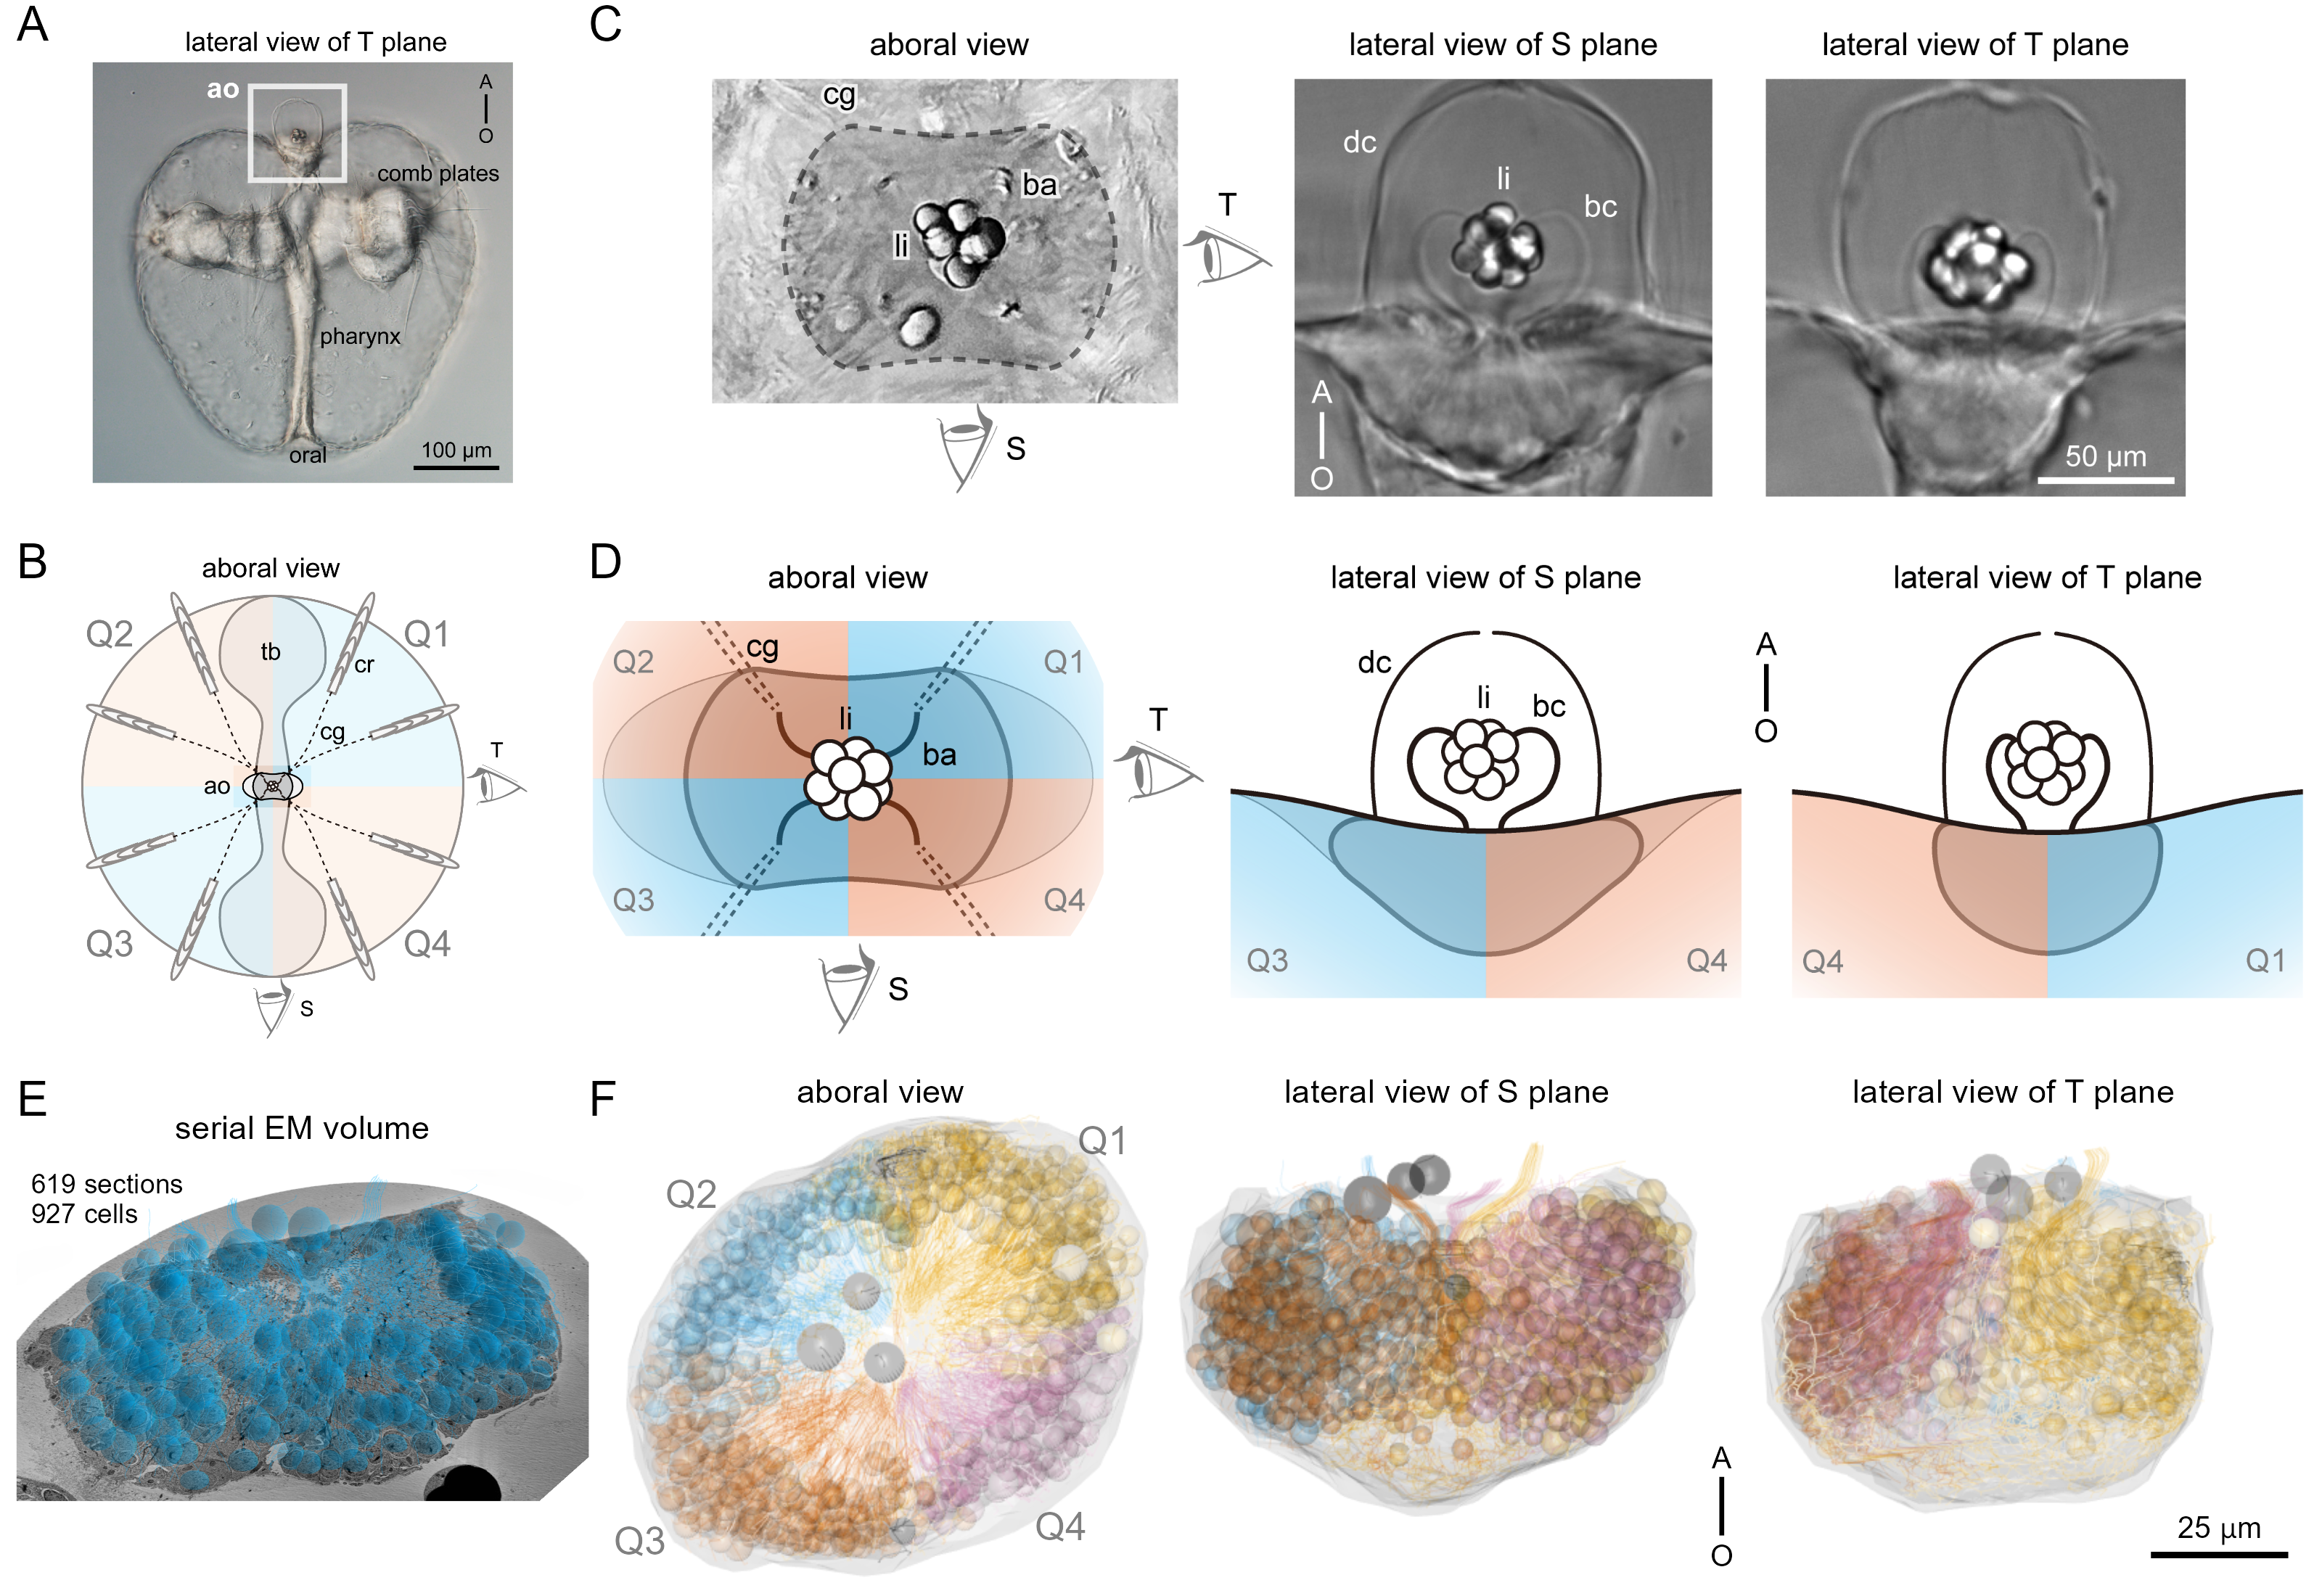
\includegraphics[width=1\textwidth,height=\textheight]{figures/Figure1.png}

}

\caption{\textbf{Figure 1. Title fig 1} pic of a larva, boxed region of
AO, schematic, catmaid pic with slice, dimensions, quadrants, regions,
(A) legend (B) legend.}

\end{figure}%

\subsubsection{Identification of Synaptic Structures in Syncytium
Neurons}\label{identification-of-synaptic-structures-in-syncytium-neurons}

Classical neural staining techniques do not provide clear images of the
neurons at the aboral pole. However, ultrastructural studies have
provided morphological evidence of elements resembling neurons, based on
synaptic structures, located on the epithelial floor of the apical
organs (Hernandez-Nicaise, 1973; Horridge and Mackay, 1964). Based on
these findings, we identified synaptic structures characteristic of
ctenophore neurons in our data, using previously identified pre-synaptic
triad morphological features, such as single-layered vesicles, smooth
endoplasmic reticulum, and tightly packed mitochondria. In our study, we
specifically identified synaptic sites and marked mitochondria (orange)
as synaptic nodes. The regions where synaptic vesicles align were marked
as connectors (light blue arrows) between cells across the membrane.
These connectors link the synaptic nodes of the pre-synaptic
cytoskeleton to the partner nodes of the post-synaptic cytoskeleton. As
previously reported, the specialization of post-synaptic structures in
ctenophores is not apparent, so we recognized synaptic vesicle clusters
on the pre-synaptic membrane as the point of reference. Synapses were
identified as either monoadic or polyadic, with one pre-synaptic neuron
forming connections with one or multiple post-synaptic cells.

As mentioned above, following the identification of the presynaptic
structures, we reconstructed three major Syncytial neurons. Each of
these Syncytial neurons was a cell with multiple nuclei, with membranes
fused by continuous plasma membranes. These neurons are distinct in
morphology from the Syncytial subepithelial nerve net (SNN) neurons with
blebbed morphology previously reconstructed in 3D
(\textbf{Burkhardt\_2023?}). Our findings represent the second
documented discovery of Syncytial neurons in ctenophores. Furthermore,
these neurons exhibited clear morphological differences when compared to
other sensory cells reported in the same study, such as mesogleal
neurons and sensory cells with presynaptic structures and cilia (types
1-4)(\textbf{Burkhardt\_2023?}). Based on their distinct spatial
relationships, we were able to classify these three Syncytial neurons
into two categories. The first type is a larger ``AO neuron\_Q1234,''
which possesses four (or possibly six?) nuclei spanning four quadrants.
It contained X presynaptic structures. The second type consists of ``AO
neuron\_Q12'' and ``AO neuron\_Q34,'' each having two nuclei spanning
two quadrants, and each containing X presynaptic structures.

\begin{figure}[H]

{\centering 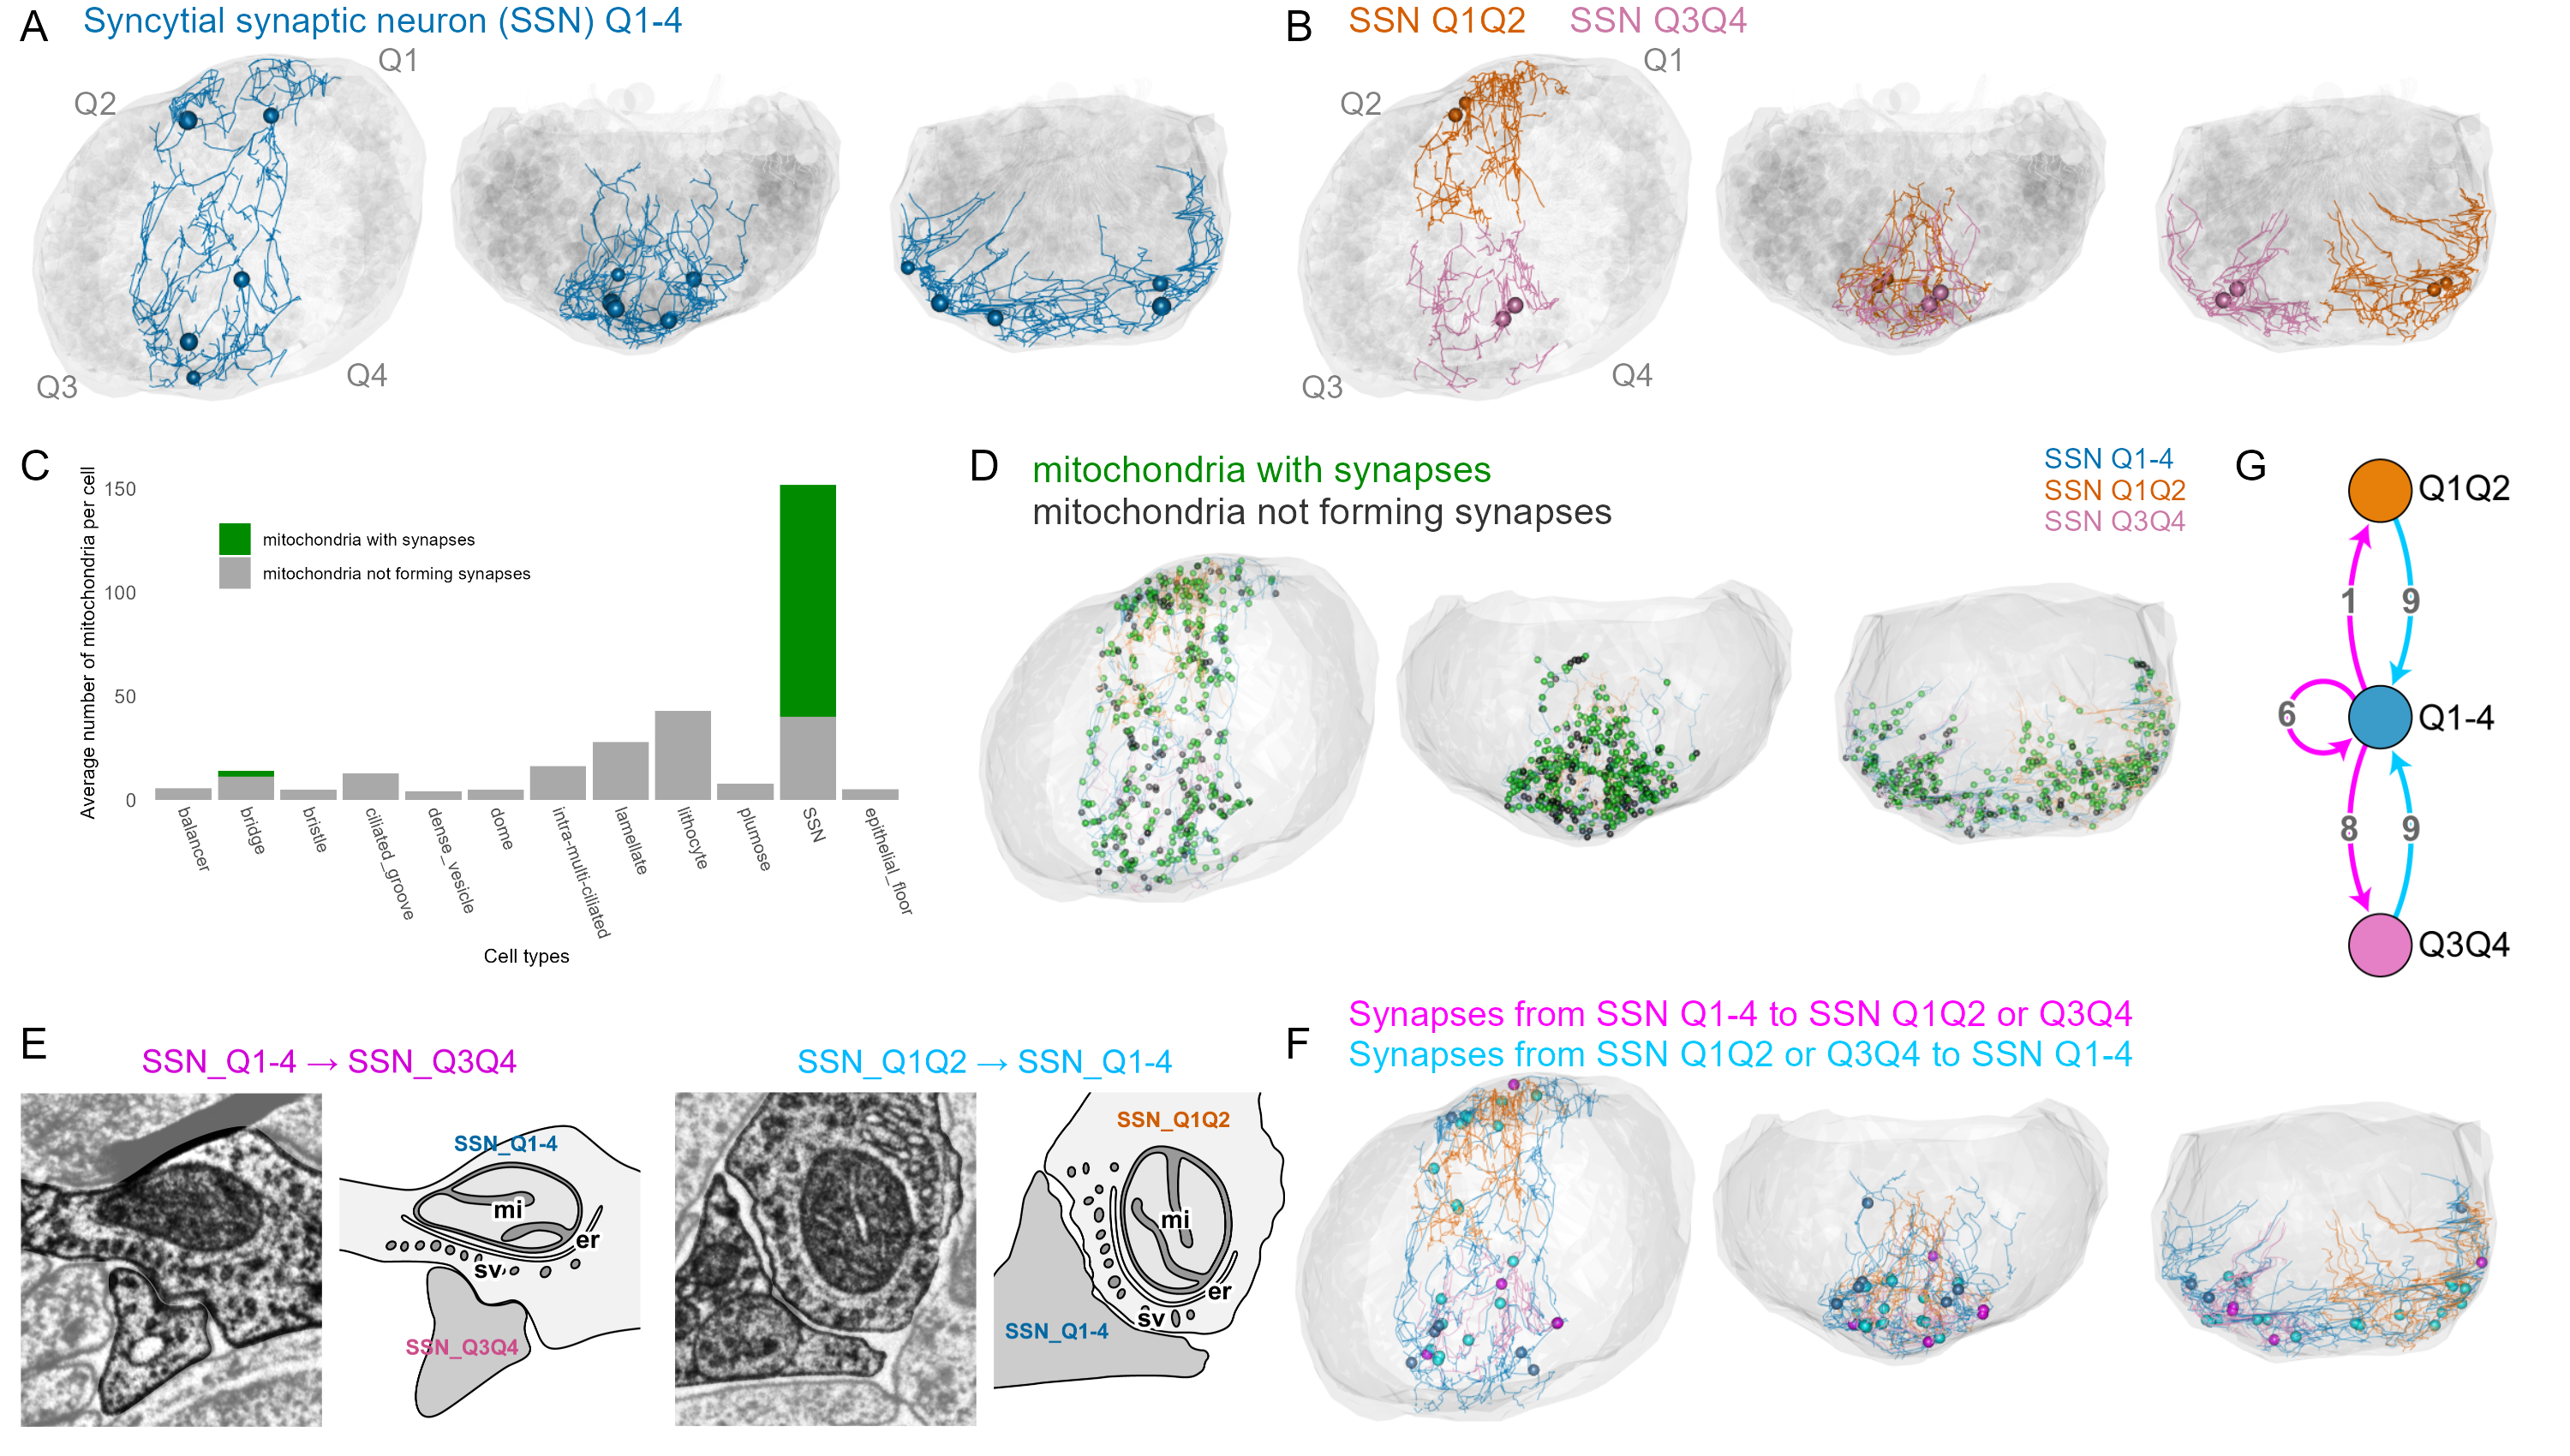
\includegraphics[width=1\textwidth,height=\textheight]{figures/Figure2.png}

}

\caption{\textbf{Figure 2. Title fig 2} pic of a larva, boxed region of
AO, schematic, catmaid pic with slice, dimensions, quadrants, regions,
(A) legend (B) legend.}

\end{figure}%

\subsubsection{Identification the Gravity-Sensitive Neural Circuit via
the Syncytial Neurons
Network}\label{identification-the-gravity-sensitive-neural-circuit-via-the-syncytial-neurons-network}

We discovered that AO neurons form synaptic connections with each other,
and that AO neuron\_Q1234 forms self-synapses, or ``autapses.'' To our
knowledge, previous reports have not identified synaptic connections
between subepithelial nerve net (SNN) neurons. Thus, our results
represent the first report of synaptic connectivity between neurons in
the apical organ, forming a network in ctenophores (subject to
confirmation). These AO neuron networks were found to form many
presynaptic structures in relation to the gravity-sensing balancer
cells.

Balancer cells are monociliated cells, and their cilia protrude longer
than those of other monociliated cells. Moreover, the cilia of balancer
cells are bundled into four groups at the center of the apical organ,
forming a compound cilium. Based on these features, we identified and
classified the balancer cells. The cellular arrangement differed clearly
when viewed in the lateral view, sagittal plane, and tentacular plane,
with the cell bodies gathering toward the apical organ in the tentacular
plane. In each quadrant, the number of cells was as follows: Q1: 37, Q2:
32, Q3: 32, Q4: 28. Each cell contained 3 to 10 ? mitochondria.

From AO neuron\_Q1Q2, synapses were formed with 6 of the 37 balancer
cells in the Q1 region, and 8 of the 32 balancer cells in the Q2 region.
Similarly, from AO neuron\_Q3Q4, synapses were formed with 1 of the 32
balancer cells in the Q3 region, and 5 of the 28 balancer cells in the
Q4 region. AO neuron\_Q1234 formed input synapses with balancer cells in
the Q1 region (7 cells), Q2 region (11 cells), Q3 region (6 cells), and
Q4 region (10 cells). Some balancer cells received inputs from both AO
neuron\_Q1Q2 or AO neuron\_Q3Q4 and AO neuron\_Q1234. While previous
studies have suggested the presence of afferent synapses from balancer
cells to neurons (\textbf{Hernandez\_Nicaise\_1974?}), our data did not
reveal any synaptic inputs from balancer cells to AO neurons. However,
we identified ``bridge cells'' that actively formed input synapses with
AO neurons, highlighting their potential role in the network.

\begin{figure}[H]

{\centering 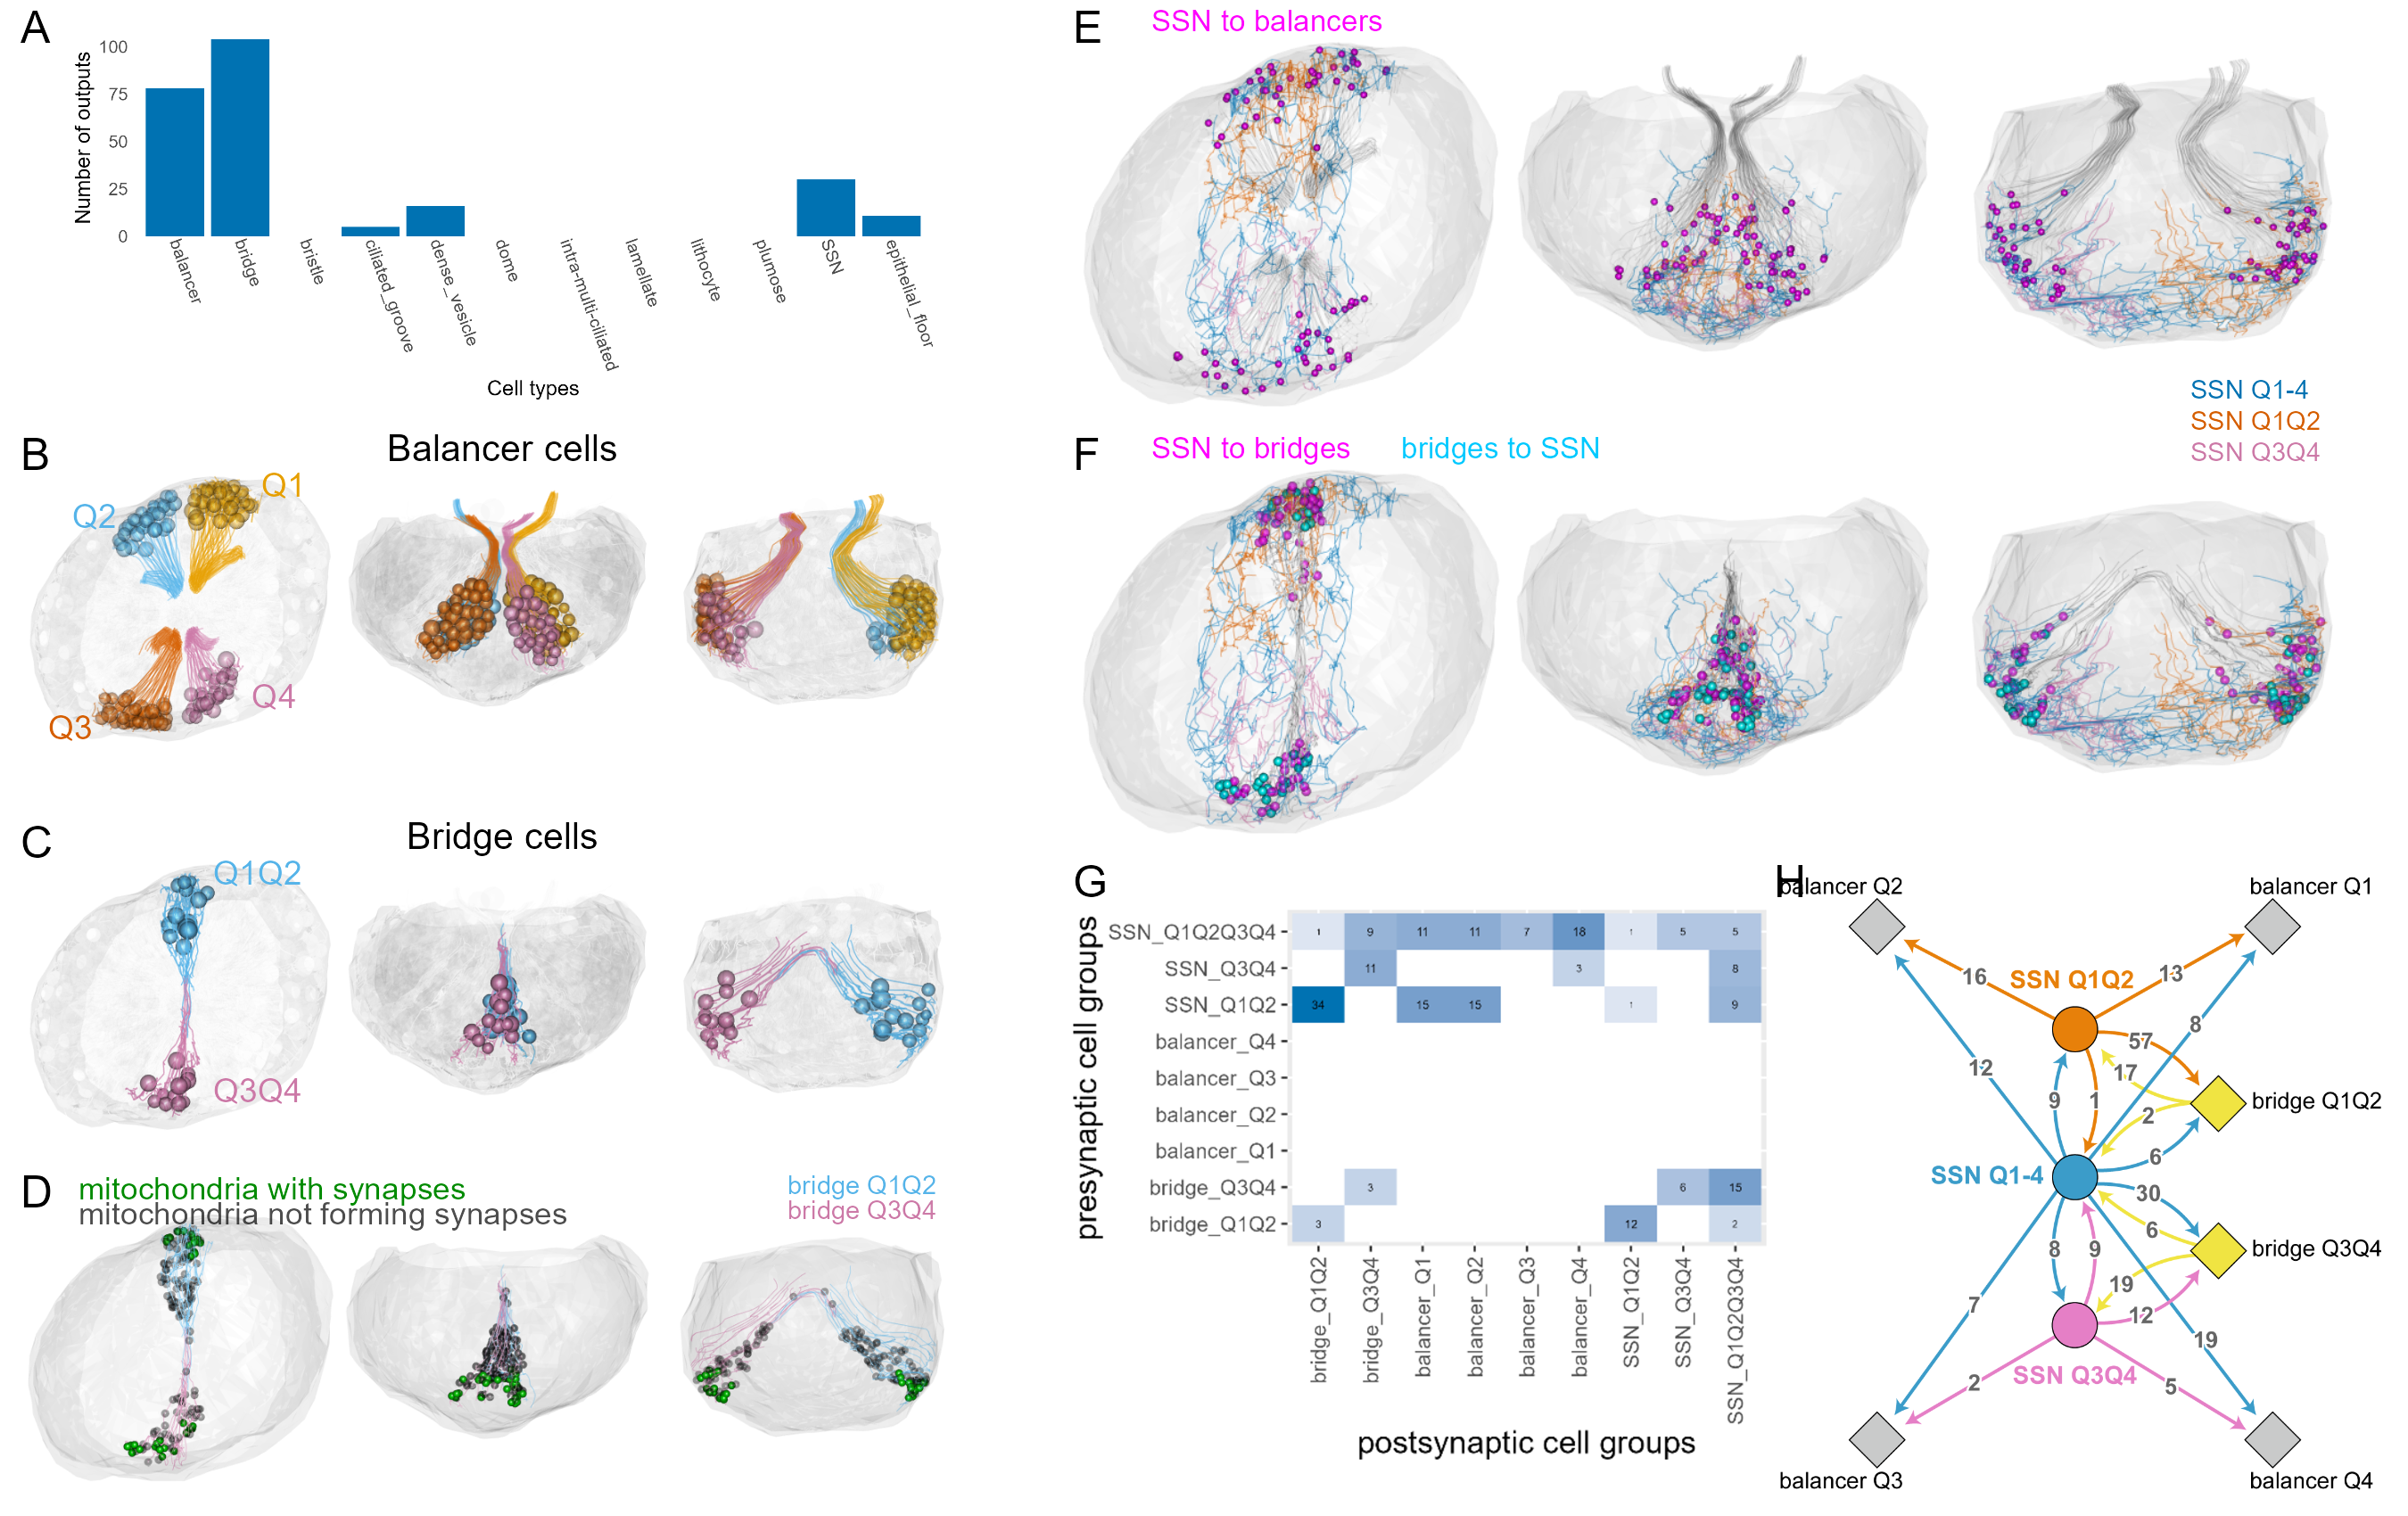
\includegraphics[width=1\textwidth,height=\textheight]{figures/Figure3.png}

}

\caption{\textbf{Figure 3. Title fig 3} pic of a larva, boxed region of
AO, schematic, catmaid pic with slice, dimensions, quadrants, regions,
(A) legend (B) legend.}

\end{figure}%

\subsubsection{Identification of Neuron-like Bridge Cells Forming
Afferent Synapses in the Gravity-Sensitive Neural
Circuit}\label{identification-of-neuron-like-bridge-cells-forming-afferent-synapses-in-the-gravity-sensitive-neural-circuit}

From our data, we identified several cell groups that form multiple
afferent synapses with AO neurons. These cells, based on their
morphological features, were found to be the bridge cells first
described by Tamm et al.~in 2002 (\textbf{Tamm\_and\_Tamm\_2002?}).
These cells are characterized by bundles of elongated processes filled
with microtubules that arch over the epithelial layer, resembling a
bridge. They originate from the base of paired balancer cells along the
tentacle surface and extend across the sagittal plane toward the base of
the opposite balancer cells. In regions where the mitochondria of the
bridge cells are localized (approximately 30\%), a presynaptic triad
structure, similar to that of AO neurons, was found, containing synaptic
vesicles and smooth endoplasmic reticulum.

Our three-dimensional reconstruction data revealed that the bridge cells
form two distinct cell groups across the sagittal plane, between the
Q1Q2 and Q3Q4 regions. In the Q1Q2 region, 14 cells were identified,
while in the Q3Q4 region, 12 cells were identified, totaling 26 bridge
cells. Nearly all of these bridge cells (25 out of 26) exhibited
afferent synapses from AO neurons. For bridge cells located in the Q1Q2
region, synaptic inputs came primarily from AO neuron\_Q1Q2 (11 cells),
AO neuron\_Q1234 (1 cell), or both (2 cells). For bridge cells located
in the Q3Q4 region, synaptic inputs were received from AO neuron\_Q3Q4
(1 cell), AO neuron\_Q1234 (7 cells), or both (1 cell). In other words,
bridge cells in the Q1Q2 region mainly received input from AO
neuron\_Q1Q2, while those in the Q3Q4 region received input primarily
from AO neuron\_Q1234, showing a distinct pattern of input in the two
regions.

Some bridge cells also formed afferent synapses with AO neurons. For
example, bridge cells in the Q1Q2 region formed synapses with AO
neuron\_Q1Q2 (3 cells) or both AO neuron\_Q1Q2 and AO neuron\_Q1234 (2
cells). Bridge cells in the Q3Q4 region formed synapses with AO
neuron\_Q3Q4 (1 cell) or AO neuron\_Q1234 (6 cells). A notable
difference was observed between the Q1Q2 and Q3Q4 regions in the
proportion of synaptic inputs from bridge cells to AO neurons.

Interestingly, in both regions, bridge cells also formed synapses with
adjacent bridge cells. However, no synaptic input was found from bridge
cells across the sagittal plane to those in the opposite region. To
analyze the grouped synaptic connectivity graph, we classified cell
types within each region, collapsed cells of the same type into a single
node, summed the number of synapses, and explored directed pathways to
effectors (balancer cell groups). The results revealed a feedback
pathway from AO neurons through the synaptic connections formed by
bridge cells, thereby shedding light on the neural circuit structure
involving these cells.

\begin{figure}[H]

{\centering 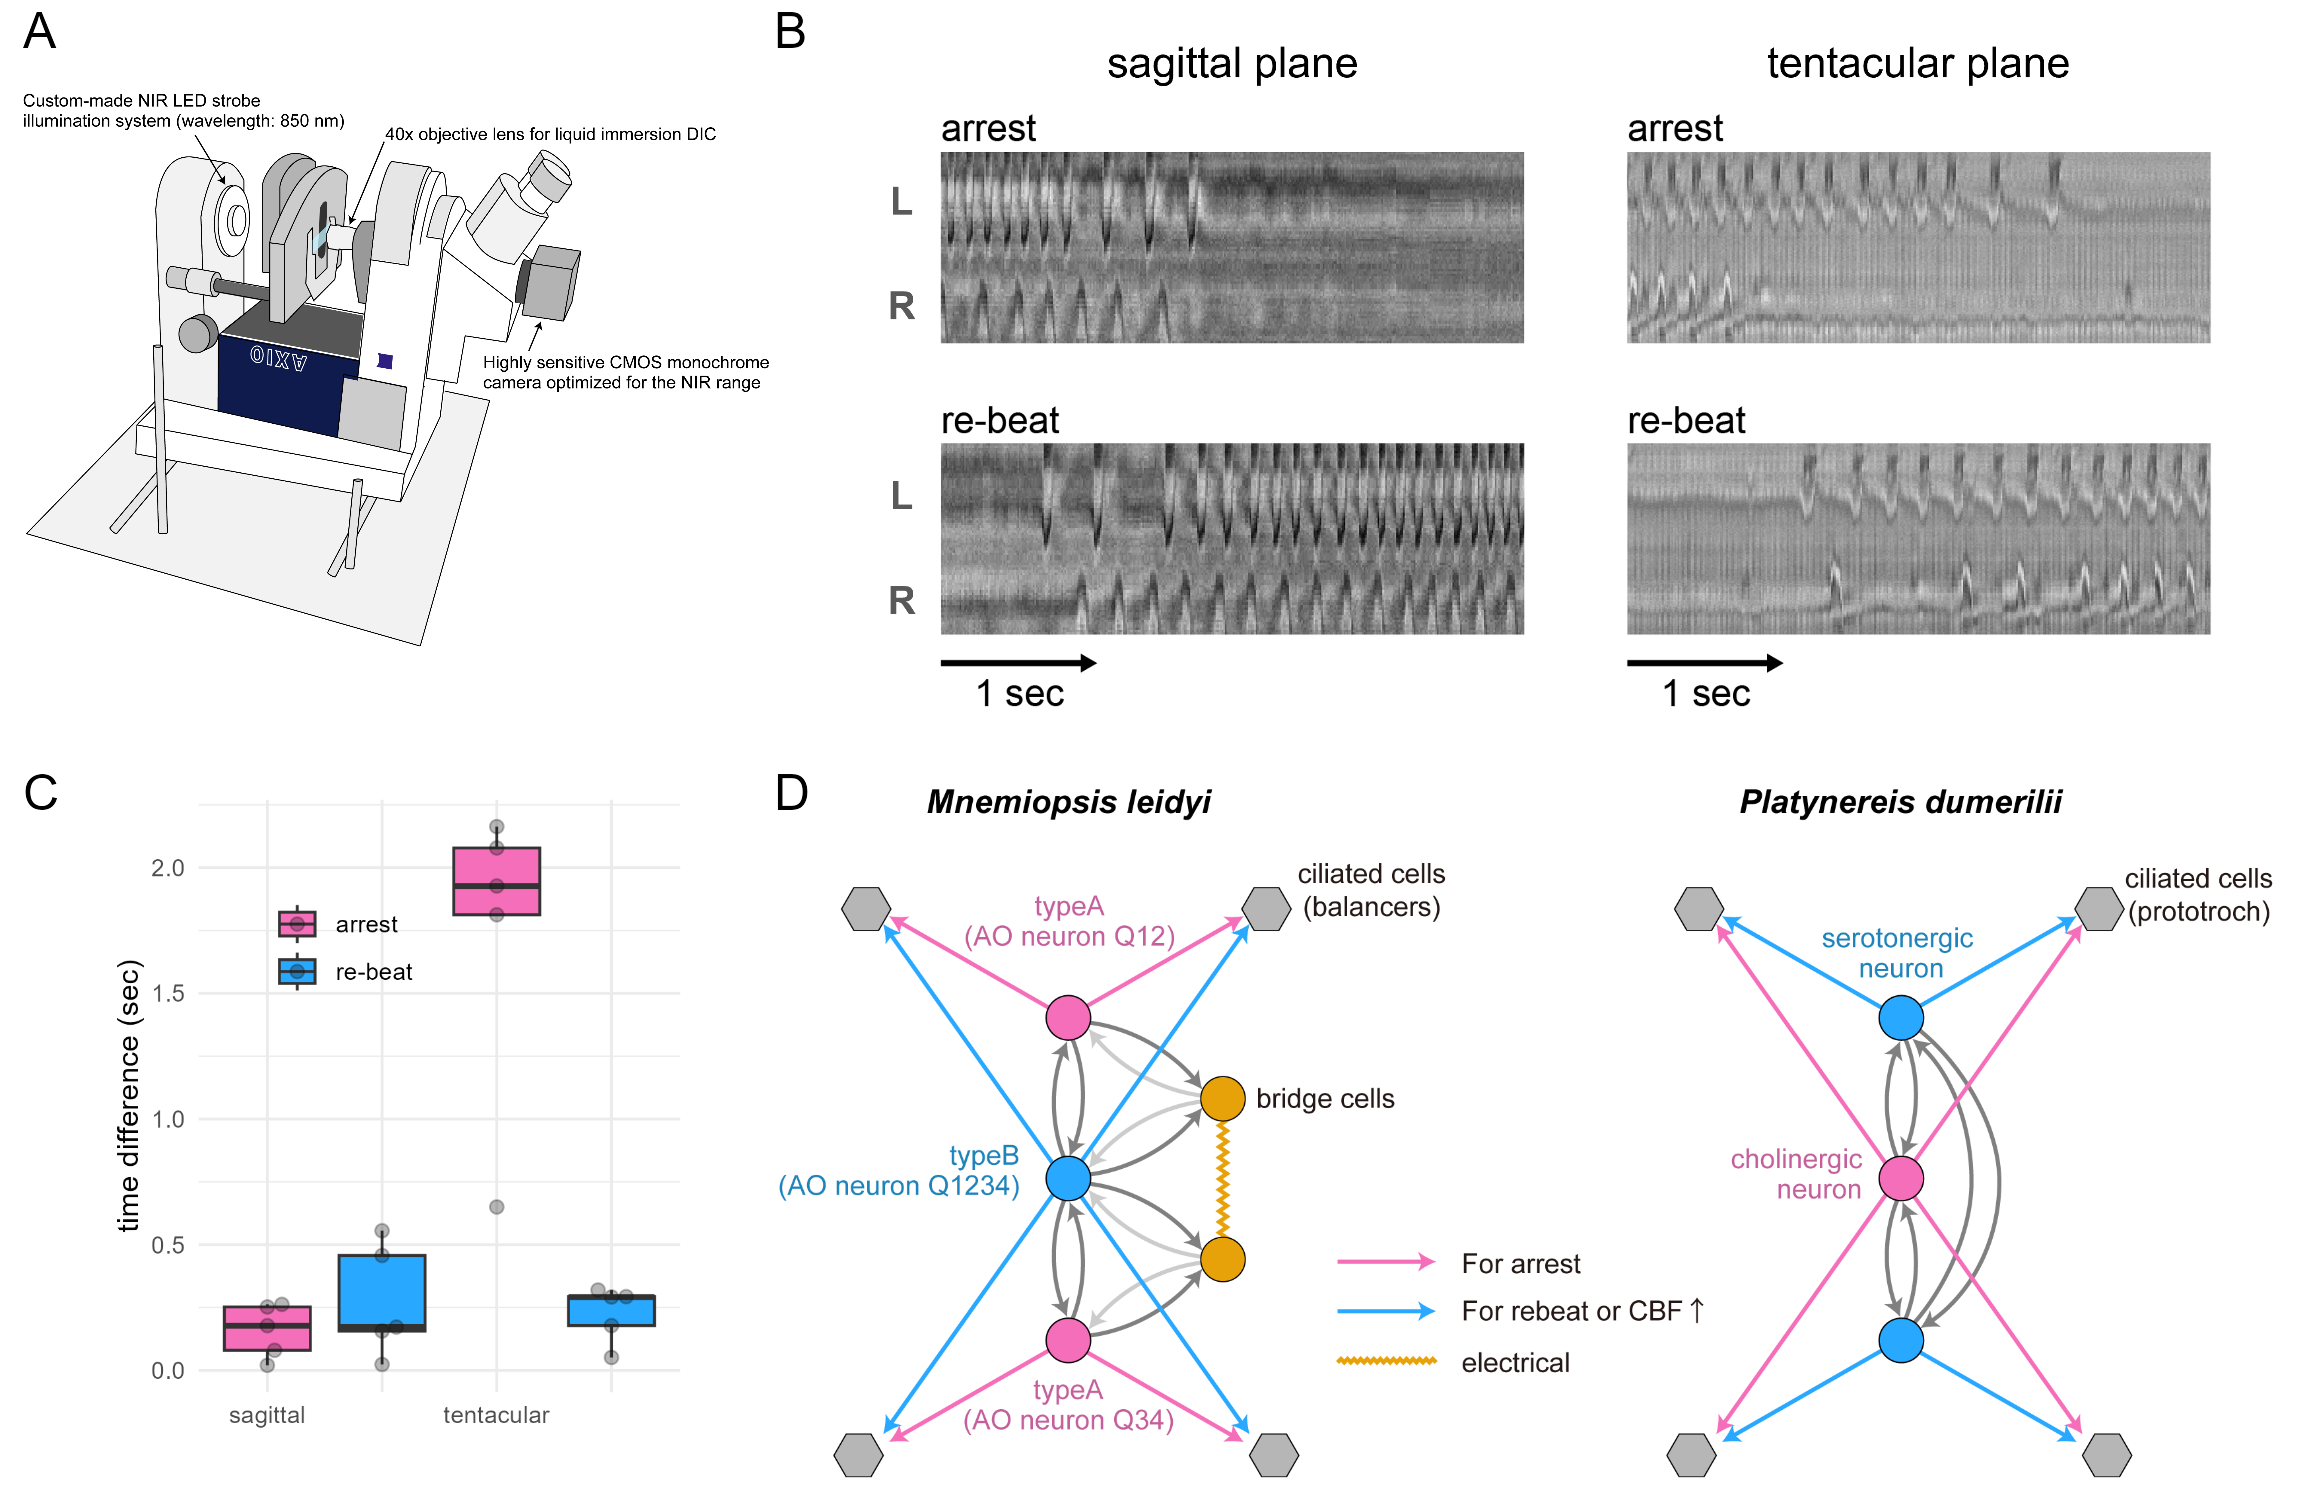
\includegraphics[width=1\textwidth,height=\textheight]{figures/Figure4.png}

}

\caption{\textbf{Figure 4. Title fig 4} pic of a larva, boxed region of
AO, schematic, catmaid pic with slice, dimensions, quadrants, regions,
(A) legend (B) legend.}

\end{figure}%

\subsection{Discussion}\label{discussion}

\subsection{Materials and Methods}\label{materials-and-methods}

\subsection{Acknowledgements}\label{acknowledgements}

We would like to thank the Jekely lab for the R project template
(\url{https://github.com/JekelyLab/new_paper_template}) we used to write
this paper. This work was funded by \ldots{} JSPS\ldots{} ERC.. Others
\ldots{}

\subsection{References}\label{references}

\subsection{Sourcing code and working with
variable}\label{sourcing-code-and-working-with-variable}

The `analysis/scripts/statistics\_for\_paper.R' script is sourced and it
runs but the output is not included in the knitted output. But we can
access the variables defined in the sourced script simply by adding ` r
var\_name ` between ` backticks, in this case max\_PRC value is (now
this number comes from our sourced script).

If we update the data, the script can recalculate the variable we want
to refer to in the text and update the number.

\phantomsection\label{refs}
\begin{CSLReferences}{1}{0}
\bibitem[\citeproctext]{ref-aronova1974electron}
Aronova M. 1974. Electron microscopic observation of the aboral organ of
ctenophora. I. The gravity receptor. \emph{Zeitschrift fur
mikroskopisch-anatomische Forschung} \textbf{88}:401--412.

\bibitem[\citeproctext]{ref-Hernandez_Nicaise_1973}
Hernandez-Nicaise M-L. 1973. The nervous system of ctenophores III.
Ultrastructure of synapses. \emph{Journal of Neurocytology}
\textbf{2}:249--263.
doi:\href{https://doi.org/10.1007/bf01104029}{10.1007/bf01104029}

\bibitem[\citeproctext]{ref-Horridge_1964}
Horridge GA, Mackay B. 1964. Neurociliary synapses in pleurobrachia
(ctenophora). \emph{Journal of Cell Science} \textbf{S3-105}:163--174.
doi:\href{https://doi.org/10.1242/jcs.s3-105.70.163}{10.1242/jcs.s3-105.70.163}

\bibitem[\citeproctext]{ref-Noda_2014}
Noda N, Tamm SL. 2014. Lithocytes are transported along the ciliary
surface to build the statolith of ctenophores. \emph{Current Biology}
\textbf{24}:R951--R952.
doi:\href{https://doi.org/10.1016/j.cub.2014.08.045}{10.1016/j.cub.2014.08.045}

\bibitem[\citeproctext]{ref-Tamm_2014}
Tamm SL. 2014. Formation of the statolith in the ctenophore mnemiopsis
leidyi. \emph{The Biological Bulletin} \textbf{227}:7--18.
doi:\href{https://doi.org/10.1086/bblv227n1p7}{10.1086/bblv227n1p7}

\bibitem[\citeproctext]{ref-Tamm_2002}
Tamm SL, Tamm S. 2002. Novel bridge of axon‐like processes of epithelial
cells in the aboral sense organ of ctenophores. \emph{Journal of
Morphology} \textbf{254}:99--120.
doi:\href{https://doi.org/10.1002/jmor.10019}{10.1002/jmor.10019}

\end{CSLReferences}




\end{document}
